%!TEX root = ../main.tex
% aspell --mode=tex --lang=it check 01-spazi_campionari_sigma-algebre_probabilita.tex

\ParteEsercizi

\Esercizio{}

Determinare un adeguato spazio campionario per ciascuno dei seguenti esperimenti aleatori.
\begin{enumerate}
	\item Il lancio di una moneta ripetuto $n$ volte.
	\item Il lancio simultaneo di $n$ monete tutte uguali tra loro.
	\item Il lancio di una moneta al minuto, senza mai fermarsi.
	\item L'estrazione di una carta da un mazzo di $10$ e lancio di una moneta.
	\item L'estrazione dei cinque numeri vincenti sulla ruota di Milano del Gioco del Lotto, ossia estrazione casuale di cinque tra i numeri naturali da $1$ a $90$.
	\item L'estrazione, una dopo l'altra, delle prime $20$ carte di un mazzo da $40$.
	\item La misurazione della frazione di tempo impiegata per risolvere il cubo di Rubik, rispetto a un tempo massimo assegnato e partendo da una configurazione casuale.
\end{enumerate}

\Esercizio{}

Una moneta viene lanciata due volte. Antonio vince se al primo lancio esce testa mentre Benedetto vince se al secondo lancio esce croce.
\begin{enumerate}
	\item Determinare il più piccolo spazio campionario che descrive tutti i possibili esiti dell'esperimento.
	\item Descrivere in termini dei sottoinsiemi dello spazio campionario i seguenti eventi:
	\begin{enumerate}
		\item \event{Antonio vince},
		\item \event{Benedetto vince},
		\item \event{Antonio non vince},
		\item \event{Benedetto non vince},
		\item \event{Antonio e Benedetto vincono entrambi},
		\item \event{vince Antonio ma non Benedetto},
		\item \event{vince Benedetto ma non Antonio},
		\item \event{almeno uno dei due vince},
		\item \event{nessuno dei due vince},
		\item \event{vince soltanto uno dei due},
		\item \event{esce testa al primo lancio ed esce croce al primo lancio},
		\item \event{esce testa o croce al secondo lancio}.
	\end{enumerate}
\end{enumerate}

\Esercizio{}

Sia $(\Omega ,\Ac)$ uno spazio di probabilità e siano $A$, $B$ e $C$ tre eventi appartenenti ad $\Ac$. Esprimere attraverso operazioni insiemistiche i seguenti eventi associati ad $A$, $B$ e $C$:
\begin{enumerate}
	\item almeno un evento si verifica,
	\item al più un evento si verifica,
	\item nessun evento si verifica,
	\item tutti gli eventi si verificano,
	\item si verifica esattamente un evento,
	\item due eventi su tre si verificano.
\end{enumerate}

Tradurre in relazioni insiemistiche le seguenti relazioni fra eventi:
\begin{enumerate}[resume]
	\item $A$ implica $B$,
	\item $A$ e $C$ si escludono a vicenda,
	\item almeno un evento fra $B$ e $C$ si verifica certamente.
\end{enumerate}

Si costruisca un esempio (o anche più di uno!) di esperimento aleatorio, avendo cura di descrivere gli eventi $A$, $B$ e $C$ e gli eventi considerati nei punti precedenti.

\Esercizio{}

Sia $(\Omega ,\Ac)$ uno spazio di probabilità e siano $A$, $B$, $C$ e $D$ quattro eventi appartenenti ad $\Ac$. Esprimere attraverso operazioni insiemistiche i seguenti eventi associati ad $A$, $B$, $C$ e $D$.
\begin{enumerate}
	\item Esattamente tre eventi su quattro si verificano.
	\item Si verifica solo $C$.
	\item Si verifica solo $C$ oppure si verifica solo $D$.
	\item Almeno un evento si verifica.
\end{enumerate}

\Esercizio{}

Si osservano i risultati del lancio di una moneta e di un dado.
\begin{enumerate}
	\item Determinare uno spazio campionario $\Omega $ che descriva tutti gli esiti dell'esperimento.
	\item Determinare la $\sigma $-algebra che descrive gli eventi verificabili a fine esperimento.
\end{enumerate}

Restringere il nostro interesse alla sola moneta, significa considerare solo alcuni degli eventi descritti dalla $\sigma $-algebra del punto $2$.
\begin{enumerate}[resume]
	\item Di quali eventi si tratta? Formano una $\sigma $-algebra?
	\item Nel caso tali eventi non formino una $\sigma $-algebra, si descriva la più piccola $\sigma $-algebra generata da essi.
\end{enumerate}

\Esercizio{}

Per $k=1,2,\NN$, si consideri $\Omega =\{0,1\}^{k}$ lo spazio degli esiti di $1$, $2$ o infinite prove di Bernoulli. In tutti e tre i casi, si consideri l'evento $E=$ \event{successo alla prima prova}, e si descriva esplicitamente la $\sigma$-algebra $\Ac =\sigma (E)$.

\Esercizio{}

Si consideri $\Omega =\{0,1\}^{\NN}$, lo spazio degli esiti di infinite prove di Bernoulli. Per $k=1,2,\dots $, si considerino gli eventi:
\begin{center}
	$E_{k}=$ \event{successo alla prova $k$},
\end{center}
e si consideri la $\sigma $-algebra $\Ac =\sigma (E_{k} \mid k=1,2,\dots)$. Si individuino i seguenti eventi e se ne mostri l'appartenenza ad $\Ac$:
\begin{enumerate}
	\item \event{solo insuccessi},
	\item \event{solo la terza prova dà un successo},
	\item \event{nelle prove pari ci sono solo successi},
	\item \event{solo successi da una qualche prova in poi},
	\item \event{infiniti successi},
	\item \event{solo un numero finito di successi},
	\item \event{solo un successo}.
\end{enumerate}

\Esercizio{}

Si consideri $\Omega =\{1,\dots ,6\}^{k}$, lo spazio degli esiti di infiniti lanci di un dado. Per $l=1,\dots ,6$ e $k=1,2,\dots $ si considerino gli eventi.
\begin{center}
	$E_{k}^{l} =$ \event{faccia $l$ al lancio $k$},
\end{center}
e si consideri la $\sigma $-algebra $\Ac =\sigma \left(E_{k}^{l} \mid l=1,\dots ,6,\ k=1,2,\dots \right)$. Si individuino i seguenti eventi e se ne mostri l'appartenenza ad $\Ac$:
\begin{enumerate}
	\item esce sempre $1$ nei primi n lanci,
	\item esce sempre $5$,
	\item solo il tredicesimo lancio dà un $3$,
	\item solo risultati dispari nei lanci dispari e risultati pari nei lanci pari,
	\item sempre $3$ dal $33$-esimo lancio in poi,
	\item sempre $3$ da un qualche lancio in poi,
	\item sempre risultati dispari da un qualche lancio in poi,
	\item infiniti $6$,
	\item solo un numero finito di $2$,
	\item solo un $4$.
\end{enumerate}

\Esercizio{}

Chiara e Marco acquistano assieme uno dei $50$ biglietti di una pesca di beneficenza. Ci sono $50$ premi di cui $7$ piacciono a Chiara, $5$ a Marco e $1$ solo ad entrambi. Uno di questi premi sarà casualmente associato al loro biglietto.
\begin{enumerate}
	\item Determinare il più piccolo spazio campionario che descrive i possibili esiti della pesca di beneficenza.
	\item Descrivere in termini di sottoinsiemi dello spazio campionario gli eventi:
	\begin{enumerate}
		\item il premio piacerà a Chiara,
		\item il premio piacerà a Marco,
		\item il premio piacerà a entrambi,
		\item il premio piacerà ad almeno uno dei due,
		\item a nessuno dei due piacerà il premio,
		\item il premio piacerà a uno solo dei due.
	\end{enumerate}
	\item Dopo aver introdotto un opportuno spazio di probabilità per descrivere questo esperimento aleatorio, valutare la probabilità di tali eventi.
\end{enumerate}

\Esercizio{}

Una ditta riceve richieste di forniture, che possono essere urgenti oppure no, e richiedere la consegna in città oppure fuori città. Per una data richiesta è noto che:
\begin{itemize}
	\item la probabilità che sia una consegna fuori città è $0.4$,
	\item la probabilità che sia una consegna urgente è $0.3$,
	\item la probabilità che sia una consegna non urgente in città è $0.4$.
\end{itemize}
Dopo aver introdotto un opportuno spazio di probabilità per descrivere questo esperimento aleatorio, calcolare:
\begin{enumerate}
	\item la probabilità che sia una consegna urgente fuori città,
	\item la probabilità che sia una consegna urgente in città.
\end{enumerate}

\Esercizio{}

Dato uno spazio di probabilità $(\Omega,\Ac,\PP)$, si mostri che:
\begin{enumerate}
	\item se un evento $A$ è quasi certo, ovvero $\PP(A) =1$, allora $\PP(A\cap B) =\PP(B)$ per ogni $B\in \Ac$;
	\item se un evento $A$ implica un evento $B$, ovvero $A\subset B$, allora $\PP(A) \leq \PP(B)$.
\end{enumerate}

\Esercizio{}

Sia $(\Omega,\Ac,\PP)$ uno spazio di probabilità e siano $A$ e $B$ due eventi appartenenti ad $\Ac$, con probabilità $\PP(A) =0.4$ e $\PP(B) =0.7$, rispettivamente. Date le seguenti affermazioni dire quali sono certamente false, quali sono sempre vere, quali possono essere vere o false:
\begin{enumerate}
	\item $\PP(A\cup B) =0.4$,
	\item $\PP(A\cup B) =0.7$,
	\item $\PP(A\cup B) \geq 0.7$,
	\item $\PP(A\cup B) =1.1$,
	\item $\PP(A\cap B) =0.28$,
	\item $\PP\left(B\cap A\comp\right) \geq 0.3$,
	\item $\PP\left(A\cap B\comp\right) \leq 0.3$.
\end{enumerate}

\Esercizio{}

Si consideri $\Omega =\{0,1\}^{\NN}$, lo spazio degli esiti di infinite prove di Bernoulli. Per $k=1,2,\dots $ si considerino gli eventi
\begin{center}
	$E_{k} =$ \event{successo alla prova $k$},
\end{center}
e si consideri la $\sigma $-algebra $\Ac =\sigma (E_{k} \mid k=1,2,\dots)$. Per ogni $n=1,2,\dots $ si consideri quindi
\begin{equation*}
	A_{n} =\bigcap_{k=1}^{n} E_{k}
\end{equation*}
\begin{enumerate}
	\item Si mostri che ogni $A_{n}$ è un evento in $A$.
	\item Si dia l'interpretazione probabilistica degli eventi $A_{n}$.
	\item Si mostri che $A_{n} \supset A_{n+1}$ per ogni $n$.
	\item Si determini $\bigcap_{n} A_{n}$, si mostri che appartiene ad $A$ e se ne dia l'interpretazione probabilistica.
\end{enumerate}
Si supponga ora che $\PP(A_{n}) =\frac{1}{2^{n}}$ per ogni $n$.
\begin{enumerate}[resume]
	\item Quanto vale $\PP\left(\bigcap_{n} A_{n}\right)$?
\end{enumerate}

\Esercizio{}

Sia $\Omega =[0,1]$ e $\Ac \coloneqq \mathcal{B}([0,1])$ la $\sigma $-algebra di Borel. Si considerino, per ogni $n\in \NN$, gli insiemi $A_{n} \coloneqq \left[0,\frac{1}{n}\right] \subset \Omega $.
\begin{enumerate}
	\item Determinare gli insiemi $I$ e $U$, definiti come segue:
	\begin{equation*}
		I\coloneqq \bigcap_{n\in \NN} A_{n} \ \ \ \ \ \ \ \ U\coloneqq \bigcup_{n\in \NN} A_{n} .
	\end{equation*}
	\item Si supponga che $\PP(A_{n}) =\frac{1}{n}$ per ogni $n$. Quanto valgono $\PP(I)$ e $\PP(U)$?
\end{enumerate}

\Esercizio{$\star$}

Sia $(\Omega,\Ac,\PP)$ uno spazio di probabilità e sia $A_{n}$ con $n\in \NN$ una successione di eventi.
\begin{enumerate}
	\item Si mostri che se $\PP(A_{n}) =0$ per ogni $n\in \NN$ allora $\PP\left(\bigcup\limits_{n\in \NN} A_{n}\right) =0$.
	\item Si mostri che se $\PP(A_{n}) =1$ per ogni $n\in \NN$ allora $\PP\left(\bigcap\limits_{n\in \NN} A_{n}\right) =1$.
\end{enumerate}

\Esercizio{$\star$}

Dato $(\Omega,\Ac,\PP)$ spazio di probabilità, data $A_{n}$ successione di eventi, si provi che
\begin{equation*}
	\PP\left(\liminf_{n} A_{n}\right) \leq \liminf_{n}\PP(A_{n}) \leq \limsup_{n}\PP(A_{n})\leq \PP\left(\limsup_{n} A_{n}\right) .
\end{equation*}
Si deduca che se $A_{n}\rightarrow A$, ovvero $\liminf_{n} A_{n} =\limsup_{n} A_{n} =A$, allora $\PP(A_{n})\rightarrow \PP(A)$.

\ParteSoluzioni

\Soluzione

\todo{1, 3, 4, 5, 6, 8, 13, 14 dovrebbero essere un po' espansi}
\todo{15, 16 mancano}

\textbf{NB.} La scelta di $\Omega $ non è unica!
\begin{enumerate}
	\item $\Omega =\{0,1\}^{n} .$
	\item $\Omega =\{0,\dots ,n\}$.
	\item $\Omega =\{0,1\}^{\NN}$.
	\item $\Omega =\{1,2,3,4,5,6,7,8,9,10\} \times \{t,c\}$.
	\item Lo spazio delle combinazioni di $90$ elementi di classe $5$, ossia
	\begin{equation*}
		\Omega =\{\omega \subseteq \{1,\dots ,90\} \mid |\omega |=5\}
	\end{equation*}
	\item Lo spazio delle disposizioni di $40$ elementi di classe $20$, ossia
	\begin{equation*}
		\Omega =\{\omega =(\omega_{1} ,\dots ,\omega_{20}) \mid \omega_{i} \in \{1,\dots ,40\} \ \forall \ i,\ \omega_{i} \neq \omega_{j} \ \forall \ i\neq j\}
	\end{equation*}
	\item $\Omega =[0,1]$.
\end{enumerate}

\Soluzione

Indichiamo la coppia (esito del primo lancio, esito del secondo lancio). Poniamo inoltre
\begin{itemize}
	\item $A=$ \event{Antonio vince}
	\item $B=$ \event{Benedetto vince}
\end{itemize}

Vediamo la soluzione dell'esercizio.
\begin{enumerate}
	\item $\Omega =\{(t,t) ,(t,c) ,(c,t) ,(c,c)\}$
	\item
	\begin{enumerate}
		\item $A=\{(t,t) ,(t,c)\}$
		\item $B=\{(t,c) ,(c,c)\}$
		\item $A\comp$
		\item $B\comp$
		\item $A\cap B=\{(t,c)\}$
		\item $A\cap B\comp$
		\item $A\comp \cap B$
		\item $A\cup B$
		\item $A\comp \cap B\comp =\{(c,t)\}$
		\item $\left(A\cap B\comp\right) \cup \left(A\comp \cap B\right) =\{(t,t) ,(c,c)\}$
		\item $\emptyset $
		\item $\Omega $
	\end{enumerate}
\end{enumerate}

\Soluzione

\begin{enumerate}
	\item $A\cup B\cup C$
	\item $\left(A\cap B\comp \cap C\comp\right) \cup \left(A\comp \cap B\cap C\comp\right) \cup \left(A\comp \cap B\comp \cap C\right) \cup \left(A\comp \cap B\comp \cap C\comp\right)$
	\item $\left(A\comp \cap B\comp \cap C\comp\right)$
	\item $(A\cap B\cap C)$
	\item $\left(A\cap B\comp \cap C\comp\right) \cup \left(A\comp \cap B\cap C\comp\right) \cup \left(A\comp \cap B\comp \cap C\right)$
	\item $\left(A\comp \cap B\cap C\right) \cup \left(A\cap B\comp \cap C\right) \cup \left(A\cap B\cap C\comp\right)$
	\item $A\subset B$
	\item $A\cap C=\emptyset $
	\item $B\cup C=\Omega $
\end{enumerate}

\Soluzione

\begin{enumerate}
	\item $\left(A\cap B\cap C\cap D\comp\right) \cup \left(A\cap B\cap C\comp \cap D\right) \cup \left(A\cap B\comp \cap C\cap D\right) \cup \left(A\comp \cap B\cap C\cap D\right)$
	\item $A\comp \cap B\comp \cap C\cap D\comp$
	\item $\left(A\comp \cap B\comp \cap C\cap D\comp\right) \cup \left(A\comp \cap B\comp \cap C\comp \cap D\right)$
	\item $A\cup B\cup C\cup D$
\end{enumerate}

\Soluzione

\begin{enumerate}
	\item $\Omega =\{t,c\} \times \{1,\dots ,6\}$
	\item $A=2^{\Omega }$
	\item Gli eventi $T=\{(t,k) \mid k=1,\dots ,6\}$ e $C=\{(c,k) \mid k=1,\dots ,6\}$. Non formano una $\sigma $-algebra.
	\item $\sigma (T,C) =\{T,C,\emptyset ,\Omega \}$.
\end{enumerate}

\Soluzione

$A=\sigma (E) =\left\{E,E\comp ,\emptyset ,\Omega \right\}$.

\Soluzione

\begin{enumerate}
	\item $\bigcup\limits_{k=1}^{\infty } E_{k}\comp$\\
	$\Ac$: $E_{k} \in \Ac \forall k\implies  E_{k}\comp \in \Ac \forall k\implies  \bigcap\limits_{k=1}^{\infty } E_{k}\comp \in \Ac$
	\item $E_{3} \cap \bigcap\limits_{k\neq 3} E_{k}\comp$
	\item $\bigcap\limits_{k=1}^{\infty } E_{2k}$
	\item $\bigcup\limits_{n=1}^{\infty }\bigcap\limits_{m\geq n} E_{m} =:\liminf_{n} E_{n}$
	\begin{oss}
		\begin{align*}
			\omega \in \liminf_{n} E_{n} & \ \ \iff \ \ \omega \in \bigcup_{n=1}^{\infty }\bigcap_{m\geq n} E_{m}\\
			 & \ \ \iff \ \ \exists \overline{n} \in \NN :\ \omega \in \bigcap_{m\geq \overline{n}} E_{m}\\
			 & \ \ \iff \ \ \exists \overline{n} \in \NN :\ \omega \in E_{m} \forall m\geq \overline{n}
		\end{align*}
		i.e. $\omega $ sta in tutti gli $E_{m}$ tranne al più un numero finito di essi.\\
		i.e. ho successi in tutte le prove al più un numero finito di esse.
	\end{oss}
	\item $\bigcap\limits_{n=1}^{\infty }\bigcup\limits_{m\geq n} E_{m} =:\limsup_{n} E_{n}$
	\begin{oss}
		\begin{align*}
			\omega \in \limsup_{n} E_{n} & \ \ \iff \ \ \omega \in \bigcap_{n=1}^{\infty }\bigcup_{m\geq n} E_{m}\\
			 & \ \ \iff \ \ \forall n\in \NN ,\ \omega \in \bigcup_{m\geq n} E_{m}\\
			 & \ \ \iff \ \ \forall n\in \NN \ \ \exists \overline{m} :\ \omega \in E_{\overline{m}}
		\end{align*}
		i.e. $\omega $ sta in $E_{m}$ per infiniti $n\in \NN$.\\
		i.e. ho infiniti successi.
	\end{oss}
	\item $\left(\liminf\limits_{n} E_{n}\right)\comp =\underbrace{\left(\bigcup\limits_{n=1}^{\infty }\bigcap\limits_{m\geq n} E_{m}\right)\comp =\bigcap\limits_{n=1}^{\infty }\bigcup\limits_{m\geq n} E_{m}\comp}_{\text{Leggi di De Morgan}} =:\limsup\limits_{n} E_{n}\comp$
	\item $\bigcup\limits_{l\in \NN}\left(E_{l} \cap \bigcap\limits_{k\neq l} E_{k}\comp\right)$
\end{enumerate}

\Soluzione

Sia $D_{k} =E_{k}^{1} \cup E_{k}^{3} \cup E_{k}^{5} \in \Ac$ e sia $P_{k} =E_{k}^{2} \cup E_{k}^{4} \cup E_{k}^{6} =D_{k}\comp \in \Ac$.
\begin{enumerate}
	\item $\bigcap\limits_{k=1}^{n} E_{k}^{1} \in \Ac$,
	\item $\bigcap\limits_{k\geq 1} E_{k}^{5} \in \Ac$,
	\item $E_{13}^{3} \cap \left(\bigcap\limits_{k\neq 13}\left[\left(E_{k}^{3}\right)\comp\right]\right) \in \Ac$,
	\item $\left(\bigcap\limits_{k\geq 0} D_{2k+1}\right) \cap \left(\bigcap\limits_{k\geq 1} P_{2k}\right) \in \Ac$,
	\item $\bigcap\limits_{k\geq 33} E_{k}^{3} \in \Ac$,
	\item $\liminf_{k} E_{k}^{3} \in \Ac$,
	\item $\liminf_{k} D_{k} \in \Ac$,
	\item $\limsup_{k} E_{k}^{6} \in \Ac$,
	\item $\left(\liminf_{k}\left(E_{k}^{2}\right)\right)\comp \in \Ac$,
	\item $\bigcup_{n}\left(E_{n}^{4} \cap \left(\bigcap_{k\neq n}\left( E_{k}^{4}\right)\comp\right)\right) \in \Ac$.
\end{enumerate}

\Soluzione

\begin{enumerate}
	\item Ricordiamo che lo spazio campionario $\Omega $ è definito come l'insieme dei possibili esiti (elementari). Intuitivamente:
	\begin{itemize}
		\item se conduciamo un dato esperimento, $\Omega $ è l'insieme di tutti i possibili esiti di tale esperimento
		\item condurre un esperimento si traduce quindi nell'estrarre un $\omega \in \Omega $.
	\end{itemize}

Inoltre, $\Omega $ non è unico, al più è unico l'$\Omega $ \textit{minimale}, ricordando che \textit{minimale}, e quindi \textit{elementare}, dipende da ciò che si stabilisce di voler controllare e descrivere. In questo caso l'esperimento che si fa deve tener conto di tutti i possibili esiti della pesca di beneficenza, i.e. $50$ possibili diversi premi. Si ha $\Omega =\{1,\dots ,50\} =$ esiti elementari per Marco e Chiara.
	\item Ricordiamo che:
	\begin{itemize}
		\item un \textit{evento} è un fatto per il quale a \textit{fine} esperimento si può dire se si è verificato o no.
		\item nel paradigma delle estrazioni da $\Omega $, un evento si verifica se pesco certi $\omega $, non si verifica se pesco altri $\omega $.
	\end{itemize}

	Chiamo $C,M$ i seguenti eventi
	\begin{itemize}
		\item $C=$ \event{il premio piace a Chiara} $=\{1,\dots ,7\}$
		\item $M=$ \event{il premio piace a Marco} $=\{7,\dots ,11\}$ (ci deve essere un elemento comune)
	\end{itemize}

\begin{oss}
Non è necessario introdurre esplicitamente $\Omega $, possiamo fare tutto in maniera astratta. Le informazioni rilevanti sono le seguenti:
\begin{equation*}
(\Omega ,\Ac) \ \ \ \ |\Omega| =50\ \ \ \ C,M\ \ \ \ \text{tali che} \ \ \ \ C,M\in \Ac ,| C| =7,| M| =5
\end{equation*}
\end{oss}
\begin{enumerate}
	\item $C$
	\item $M$
	\item $C\cap M$
	\item $C\cup M$
	\item $(C\cup M)\comp$
	\item $(C\cup M) \setminus (C\cap M)$
\end{enumerate}

	Per rispondere era necessario ricordare che le operazioni logiche tra insiemi si traducono in operazioni insiemistiche:
	\begin{align*}
		\emptyset  & =\text{evento impossibile}\\
		\Omega  & =\text{evento certo}\\
		A\comp & =\text{contrario di} \ A\\
		A\cup B & \iff A\ \text{oppure} \ B\\
		A\cap B & \iff A\ \text{e} \ B\\
		A\cap B=\emptyset  & \iff A\ \text{e} \ B\ \text{incompatibili}\\
		A\subseteq B & \iff A\ \text{implica} \ B
	\end{align*}
	\item In questo caso l'insieme degli eventi $\Omega $ è un insieme discreto (finito). La probabilità è uniforme: gli eventi equiprobabili a priori. Pertanto si ha
	\begin{equation*}
		\PP(A) =\frac{| A| }{|\Omega| } =\frac{\text{casi favorevoli}}{\text{casi possibili}}
	\end{equation*}
	Allora
	\begin{enumerate}
		\item $\PP(C) =\frac{| C| }{|\Omega| } =\frac{7}{50} =0.14$
		\item $\PP(M) =\frac{| M| }{|\Omega| } =\frac{5}{50} =0.1$
		\item $\PP(C\cap M) =\frac{1}{50} =0.02$
		\item $\PP(C\cup M) =\frac{11}{50} =0.22$
		\item $\PP\left((C\cup M)\comp\right) =1-0.22=0.78$
		\item Procediamo come segue
		\begin{align*}
			\PP((C\cup M) \setminus (C\cap M)) & \underbrace{=\PP(C\cup M) -\overbrace{\PP((C\cup M) \cap (C\cap M))}^{\PP(C\cap M)}}_{\PP(A\setminus B) =\PP(A) -\PP(A\cap B)}\\
			 & =\PP(C\cup M) -\PP(C\cap M)\\
			 & =0.22-0.02=0.2
		\end{align*}
	\end{enumerate}
\end{enumerate}

\Soluzione

\textbf{Primo Metodo.}

Introduciamo lo spazio campionario $\Omega =\{U_{c} ,U_{f} ,N_{c} ,N_{f}\}$ per indicare gli urgenti $(U)$ e in non urgenti $(N)$ rispettivamente in città $(_{c})$ e fuori città $(_{f})$. Usiamo come $\sigma $-algebra $\Ac =2^{\Omega }$. Poniamo:
\begin{itemize}
	\item $F=\{N_{f} ,U_{f}\} =$ \event{consegna fuori città}
	\item $U=\{U_{c} ,U_{f}\} =$ \event{consegna urgente}
\end{itemize}
Dalle ipotesi del problema sappiamo che:
\begin{gather*}
	\PP(F) =\PP(\{N_{f} ,U_{f}\}) =0.4\\
	\PP(U) =\PP(\{U_{c} ,U_{f}\}) =0.3\\
	\PP(\{N_{c}\}) =0.4
\end{gather*}
Ricordiamo inoltre che:
\begin{gather*}
	\PP(A\cup B) =\PP(A) +\PP(B) -\PP(A\cap B) \implies \PP(A\cap B) =\PP(A) +\PP(B) -\PP(A\cup B)
\end{gather*}
In questo modo possiamo calcolare:
\begin{enumerate}
	\item la probabilità di consegna urgente fuori città
	\begin{align*}
		\PP(\{U_{f}\}) & =\PP(F\cap U)\\
		& =\PP(F) +\PP(U) -\PP(F\cup U)\\
		& =\PP(F) +\PP(U) -\PP(\{N_{f} ,U_{f} ,U_{c}\})\\
		& =\PP(F) +\PP(U) -\PP(\Omega \setminus \{N_{c}\})\\
		& =0.4+0.3-(1-0.6)\\
		& =0.1
	\end{align*}
	\item la probabilità di consegna urgente in città
	$\PP(\{U_{c}\}) =\PP(U) -\PP(\{U_{f}\}) =0.3-0.1=0.2$
\end{enumerate}
\begin{oss}
	Per avere i valori di probabilità di tutti i mattoncini possiamo anche calcolare
	\begin{equation*}
		\PP(\{N_{f}\}) =1-\PP(\{U_{f}\}) -\PP(\{U_{c}\}) -\PP(\{N_{c}\}) =1-0.1-0.2-0.4=0.3
	\end{equation*}
	In altri termini $\{N_{f}\} ,\{U_{f}\} ,\{N_{c}\} ,\{U_{c}\}$ rappresentano una partizione di $\Omega $. Sapendo le probabilità di questi eventi, ricaviamo le probabilità di qualsiasi evento.
\end{oss}

\textbf{Secondo Metodo.}

Con questo metodo mostriamo come non sia necessario introdurre $\Omega $: è possibile fissare un arbitrario spazio di probabilità $(\Omega,\Ac,\PP)$ e definire la probabilità su specifici eventi in $\Ac$. Siano:
\begin{itemize}
	\item $C=$ \event{consegna in città}
	\item $U=$ \event{consegna urgente}
\end{itemize}

L'insieme $\Omega $ delle possibili consegne è unione dei seguenti eventi, tra loro incompatibili:
\[
	\begin{array}{lc}
			& \text{con probabilità}\\
		C\phantom{\comp} \cap U      & a\\
		C         \comp  \cap U      & b\\
		C\phantom{\comp} \cap U\comp & c\\
		C         \comp  \cap U\comp & d
	\end{array}
\]
Stiamo costruendo $\Omega $ come insieme delle possibili modalità di una richiesta. Stiamo partizionando $\Omega $.

\begin{figure}[htpb]
	\centering
	\tikzset{every picture/.style={line width=0.75pt}} %set default line width to 0.75pt        

	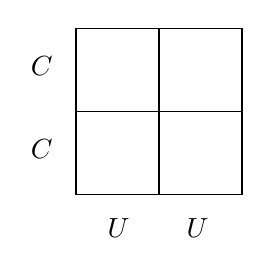
\begin{tikzpicture}[x=0.75pt,y=0.75pt,yscale=-1,xscale=1]
	%uncomment if require: \path (0,124); %set diagram left start at 0, and has height of 124

	%Shape: Square [id:dp05978656421370365] 
	\draw   (260,10) -- (340,10) -- (340,90) -- (260,90) -- cycle ;
	%Straight Lines [id:da27899061599265207] 
	\draw    (340,50) -- (260,50) ;
	%Straight Lines [id:da4092530719672025] 
	\draw    (300,90) -- (300,10) ;

	% Text Node
	\draw (237,22.4) node [anchor=north west][inner sep=0.75pt]    {$C$};
	% Text Node
	\draw (237,62.4) node [anchor=north west][inner sep=0.75pt]    {$C\comp$};
	% Text Node
	\draw (274,100.4) node [anchor=north west][inner sep=0.75pt]    {$U$};
	% Text Node
	\draw (312,100.4) node [anchor=north west][inner sep=0.75pt]    {$U\comp$};


	\end{tikzpicture}
\end{figure}
\FloatBarrier

I dati si traducono come segue:
\begin{itemize}
	\item $0.4=\PP\left(C\comp\right) =\PP\left(\left(C\comp \cap U\right) \cup \left(C\comp \cap U\comp\right)\right)=\PP\left(C\comp \cap U\right) +\PP\left(C\comp \cap U\comp\right)=b+d$
	\item $0.3=\PP(U) =\PP\left(\left(C\comp \cap U\right) \cup (C\cap U)\right)=\PP\left(C\comp \cap U\right) +\PP(C\cap U)=b+a$
	\item $0.4=\PP\left(U\comp \cap C\right) =c$
\end{itemize}

Si ricava allora:
\begin{equation*}
	a=0.2,\qquad b=0.1,\qquad c=0.4,\qquad d=0.3.
\end{equation*}
Quindi la probabilità che ci sia una consegna urgente in città è $\PP(U\cap C) =a=0.2$ e la probabilità che ci sia una consegna urgente fuori città è $\PP\left(U\cap C\comp\right) =b=0.1$.

\Soluzione

\begin{enumerate}
	\item Scriviamo $B$ come unione disgiunta di insiemi:
	\[
		B=(B\setminus A) \cup (A\cap B) =\left(B\cap A\comp\right) \cup (A\cap B)
	\]
	Dimostriamo le due disuguaglianze.
	\begin{enumerate}
		\item $\PP(B) =\overbrace{\PP\left(\left(B\cap A\comp\right) \cup (A\cap B)\right) =\underbrace{\PP\left(B\cap A\comp\right)}_{\geq 0} +\PP(A\cap B)}^{\text{perché gli insiemi sono disgiunti}} \geq \PP(A\cap B)$
		\item $\PP(A\cap B) =\PP(A) +\PP(B) -\underbrace{\PP(A\cap B)}_{\leq 1} \geq \underbrace{\PP(A)}_{=1} +\PP(B) -1=\PP(B)$
	\end{enumerate}
	Quindi abbiamo $\PP(A\cap B) =\PP(B)$.
	\item Scriviamo $B$ come unione di insiemi disgiunti: $B=A\cup (B\setminus A)$.
	\[
		\PP(B) =\PP(A\cup ( B\setminus A)) =\PP(A) +\underbrace{\PP(B\setminus A)}_{\geq 0} \geq \PP(A)
	\]
\end{enumerate}

\Soluzione

Facciamo due osservazioni per poter rispondere ai primi quesiti.
\begin{equation*}
	\begin{cases}
		\PP(A\cup B) \geq \PP(A) =0.4\\
		\PP(A\cup B) \geq \PP(B) =0.7
	\end{cases}
	\implies \boxed{\PP(A\cup B) \geq 0.7}
\end{equation*}
analogamente
\begin{equation*}
	\begin{cases}
		\PP(A\cap B) \leq \PP(A) =0.4\\
		\PP(A\cap B) \leq \PP(B) =0.7
	\end{cases}
	\implies \boxed{\PP(A\cap B) \leq 0.4}
\end{equation*}
Allora:
\begin{enumerate}
	\item F
	\item F/V (è plausibile)
	\item V
	\item F
	\item V/F (è plausibile)
	\item V, infatti
	\begin{equation*}
		\PP(B) =\PP(A\cap B) +\PP\left(B\cap A\comp\right)
	\end{equation*}
	pertanto
	\begin{equation*}
		\PP\left(B\cap A\comp\right) =\underbrace{\PP(B)}_{=0.7} -\underbrace{\PP(A\cap B)}_{\leq 0.4} \geq 0.7-0.4=0.3
	\end{equation*}
	\item V, infatti
	\begin{equation*}
		\begin{cases}
			\PP\left(A\cap B\comp\right) \leq \PP(A) =0.4\\
			\PP\left(A\cap B\comp\right) \leq \PP\left(B\comp\right) =1-\PP(B) =1-0.7=0.3
		\end{cases}
		\implies \PP\left(A\cap B\comp\right) \leq 0.3
	\end{equation*}
\end{enumerate}

\Soluzione

\begin{enumerate}
	\item Proprietà delle $\sigma $-algebre
	\item Solo successi nelle prime $n$ prove
	\item Scriviamo le relazioni insiemistiche
	\begin{align*}
		A_{n+1} \coloneqq \bigcap\limits_{k=1}^{n+1} E_{k} & =E_{k+1} \cap \underbrace{\bigcap\limits_{k=1}^{n} E_{k}}_{A_{n}} =E_{k+1} \cap A_{n} \subset A_{n}\\
		\omega \in A_{n+1} & \iff \omega \in E_{k+1} \cap A_{n}\\
		 & \iff \omega \in E_{k+1} \land \omega \in A_{n}\\
		 & \text{i.e.} \ A_{n+1} \subset A_{n} \ \forall n
	\end{align*}
	\item Scriviamo le relazioni insiemistiche
	\begin{align*}
		\bigcap\limits_{n\in \NN} A_{n} =\bigcap\limits_{n\in \NN}\bigcap\limits_{k=1}^{n} E_{k} =\bigcap\limits_{k\in \NN} E_{k} & =\text{solo successi}\\
		\omega \in \bigcap\limits_{n\in \NN} A_{n} & \iff \omega \in A_{n} \ \forall n\in \NN\\
		 & \iff \omega \in \bigcap\limits_{k=1}^{n} E_{k} \ \forall n\in \NN\\
		 & \iff \omega \in E_{k} \ \forall n\in \NN \ \forall k=1,\dots ,n\\
		 & \iff \omega \in E_{k} \ \forall k
	\end{align*}
	$\bigcap\limits_{n\in \NN} A_{n} \in \Ac$ per le proprietà delle $\sigma $-algebre.
	\item Abbiamo $A_{n} \downarrow A$ con $A\coloneqq \bigcap\limits_{n\in \NN} A_{n}$ infatti
	\[
		\begin{cases}
			A_{n+1} \subseteq A_{n} \ \forall n\\
			\bigcap_{n\in \NN} A_{n} =A.
		\end{cases}
	\]
	Per la continuità di $\PP$ dall'alto si ha $\PP(A) =\PP\left(\bigcap\limits_{n\in \NN} A_{n}\right) =\lim\limits_{n}\PP(A_{n}) =\lim\limits_{n}\frac{1}{2^{n}} =0$.
\end{enumerate}

\Soluzione

\begin{enumerate}
	\item $\forall n\in \NN \ \ \ \ A_{n} =\left[ 0,\frac{1}{n}\right)$
	\begin{figure}[htpb]
		\centering
		\tikzset{every picture/.style={line width=0.75pt}} %set default line width to 0.75pt        

		\begin{tikzpicture}[x=0.75pt,y=0.75pt,yscale=-1,xscale=1]
		%uncomment if require: \path (0,91); %set diagram left start at 0, and has height of 91

		%Straight Lines [id:da5723837040292659] 
		\draw    (142,27.5) -- (416.5,27.5) ;

		% Text Node
		\draw (159,12.4) node [anchor=north west][inner sep=0.75pt]  [font=\LARGE]  {$[$};
		% Text Node
		\draw (369,12.4) node [anchor=north west][inner sep=0.75pt]  [font=\LARGE]  {$)$};
		% Text Node
		\draw (269,12.4) node [anchor=north west][inner sep=0.75pt]  [font=\LARGE]  {$)$};
		% Text Node
		\draw (189,12.4) node [anchor=north west][inner sep=0.75pt]  [font=\LARGE]  {$)$};
		% Text Node
		\draw (158,52.4) node [anchor=north west][inner sep=0.75pt]    {$0$};
		% Text Node
		\draw (368,52.4) node [anchor=north west][inner sep=0.75pt]    {$1$};
		% Text Node
		\draw (268,52.4) node [anchor=north west][inner sep=0.75pt]    {$\frac{1}{2}$};
		% Text Node
		\draw (188,52.4) node [anchor=north west][inner sep=0.75pt]    {$\frac{1}{n}$};
		% Text Node
		\draw (229,12.4) node [anchor=north west][inner sep=0.75pt]  [font=\LARGE]  {$)$};
		% Text Node
		\draw (228,52.4) node [anchor=north west][inner sep=0.75pt]    {$\frac{1}{3}$};

		\end{tikzpicture}
	\end{figure}
	\FloatBarrier
	Osserviamo che gli insiemi $A_{n}$ sono inscatolati, i.e. $A_{n+1} \subseteq A_{n} \ \forall n$. Si ha:
	\begin{equation*}
		I=\bigcap_{n\in \NN} A_{n} \ =\{0\} \ \ \ \ \ \ \ \ U=\bigcup_{n\in \NN} A_{n} \ =[ 0,1) =A_{1}
	\end{equation*}
	\item Abbiamo $A_{n} \downarrow I$, infatti $A_{n+1} \subseteq A_{n} \ \forall n$ e $\bigcap_{n\in \NN} A_{n} =I$.\\
	Allora per la continuità dall'alto si ha $\PP(I) =\lim_{n}\PP(A_{n}) =\lim_{n}\frac{1}{n} =0$.\\
	Infine $\PP(U) =\PP([ 0,1)) =\PP(A_{1}) =1$.
\end{enumerate}

\Soluzione

Manca.

\Soluzione

Manca.